\chapter{ARTICULAÇÃO COM OS VALORES, PRINCÍPIOS E POLÍTICAS DE ENSINO DA UTFPR}

Este Capítulo é uma complementação do \autoref{chap:politicas}, apresentado a estruturação das políticas de ensino da UTFPR no âmbito do Curso de Engenharia Eletrônica, tendo como base a matriz curricular apresentada no \autoref{chap:matriz}.

\section{DESENVOLVIMENTO DA ARTICULAÇÃO ENTRE A TEORIA E A PRÁTICA}

O curso de Engenharia Eletrônica define quatro instrumentos para desenvolver a articulação entre a teoria e a prática: (i) atividades práticas em unidades curriculares, (ii) projetos práticos interdisciplinares, (iii) estágio curricular obrigatório e (iv) Trabalho de Conclusão de Curso (TCC).

Neste sentido, a matriz curricular do curso de Engenharia Eletrônica apresenta 34 (trinta e quatro) unidades curriculares que contemplam carga horária prática, totalizando \the\value{horasAP} horas de atividades práticas. Informações mais detalhadas sobre esta distribuição podem ser observadas no \autoref{qua:matriz} na \autoref{sec:matriz}, Matriz Curricular.

Além disso, os docentes são encorajados a aplicarem projetos práticos interdisciplinares, onde experiências práticas de implementação de projetos são propostas aos discentes, complementando a articulação entre teoria e prática, e inserindo a perspectiva de interdisciplinaridade no curso. Tipicamente, tais projetos são desenvolvidos nas unidades curriculares de Sistemas Digitais, Microcontroladores, Sistemas Embarcados, Medidas e Sensores e Eletrônica de Potência.

O estágio curricular obrigatório contabiliza \dadoCHT{E.1} h de atividades, podendo ser iniciado a partir do 7\textordmasculine{} período. Neste contexto, o estudante é capaz de colocar em prática todo o ensinamento recebido durante seus anos de estudo no curso, sendo acompanhado por um professor orientador e um supervisor responsável pelo estágio na empresa que o oferece. Para possibilitar um melhor aproveitamento do discente em relação ao Estágio, este PPC foi desenvolvido prevendo a redução de carga horária nos nono e décimo períodos. Desta forma, o discente tem condições de buscar oportunidades de estágio em outras regiões, dentro e/ou fora do país.

Assim como o estágio obrigatório, o TCC é capaz de colocar em prática todo o ensinamento recebido pelo discente durante o curso, sendo acompanhado por um(a) docente orientador(a). Os(as) orientadores, em consonância com a atuação do docente responsável pelas atividades de TCC, buscam sempre a realização de projetos práticos e interdisciplinares, como é caso do desenvolvimento de processos, produtos ou protótipos.

\section{DESENVOLVIMENTO DAS COMPETÊNCIAS PROFISSIONAIS}
\label{sec:comp}

Assim como citado na \autoref{sec:perf}, neste PPC são propostas seis Competências Específicas para o egresso do curso: Básica, Computação, Eletrônica, Científica, Empreendedora e Eletrotécnica. As competências são desenvolvidas gradativamente em várias unidades curriculares e em momentos distintos no decorrer do curso. Em alguns casos, unidades curriculares são comuns a mais de uma competência. As competências são desenvolvidas quando o/a estudante concluem determina trilha de unidades curriculares.

\subsection{A competência Básica}

Ao conquistar essa competência, o discente será capaz de \textbf{\compBasica}. As Unidades Curriculares necessárias para esta competência são: Introdução à Engenharia, Cálculo Diferencial e Integral 1, 2, 3 e 4B; Cálculo numérico; Probabilidade e estatística; Física 1, 2, 3 e 4; Química Básica Teórica e Experimental; Mecânica 1; Fenômenos de Transporte e Eletromagnetismo.

\subsection{A competência de Computação}

Ao conquistar essa competência, o discente será capaz de \textbf{\compComp}. As Unidades Curriculares necessárias para esta competência são: Computação 1, Fundamentos de Programação, Arquitetura e Organização de Computadores, Cálculo numérico e Sistemas Operacionais.

\subsection{A competência de Eletrônica}

Ao conquistar essa competência, o discente será capaz de \textbf{\compTron}. Para conquistar a competência de Eletrônica é necessário que o discente seja aprovado em quatro ramos de unidades curriculares que compreendem quatro áreas de atuação, sendo elas:

\begin{itemize}
    \item Circuitos Eletrônicos;
    \item Sistemas Embarcados;
    \item Processamento Digital de Sinais; e
    \item Sistemas de Controle.
\end{itemize}

As Unidades curriculares necessárias para cada área estão dispostas na \autoref{fig:copele}. Pode-se notar que em cada ramo da Competência de Eletrônica existem unidades curriculares destacadas (sublinhadas), sendo responsáveis por integrar o conhecimento de cada área área de atuação.

\begin{figure}[!htb]
    \centering
    \caption[Áreas e unidades curriculares da Competência de Eletrônica]{Áreas e unidades curriculares da Competência de Eletrônica}
    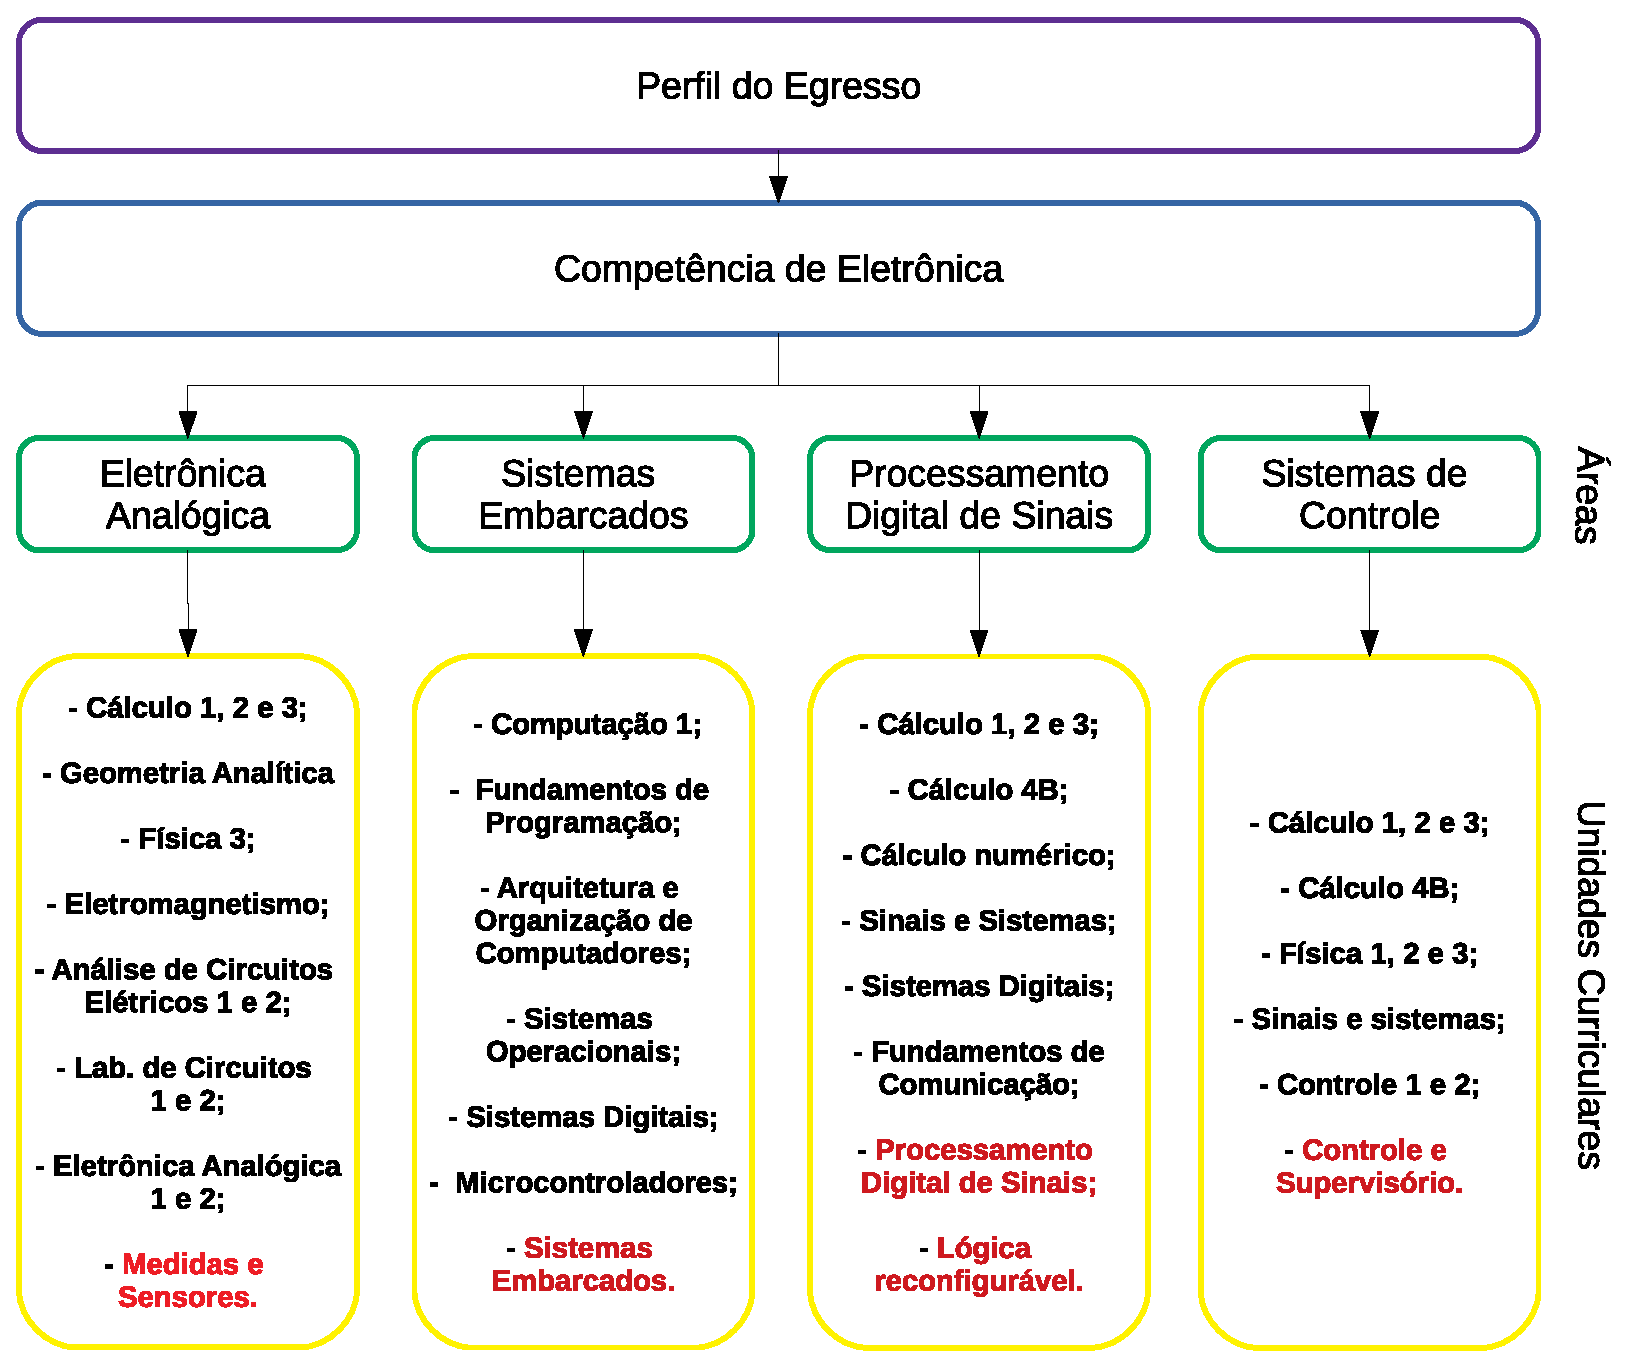
\includegraphics[width=1.0\textwidth]{Caps/Figs/comp_eletronica.eps}
    \fonte{\utf}
    \label{fig:copele}
\end{figure}

\subsection{A competência Científica}

Ao conquistar essa competência, o discente será capaz de \textbf{\compCien}. As unidades curriculares necessárias para esta competência são Metodologia da Pesquisa, Trabalho de Conclusão de Curso 1 e Trabalho de Conclusão de Curso 2. Cabe destacar que para a estruturação dessa competência cada discente precisa aplicar os conhecimentos e as demais competências adquiridas no decorrer do curso.

\subsection{A competência Empreendedora}

Ao conquistar essa competência, o discente será capaz de \textbf{\compEmp}. Para a estruturação da competência, o discente precisa cursar algumas unidades curriculares optativas do ciclo de humanidades: Gestão de Projetos, Empreendedorismo, Ciências do Ambiente e uma unidade curricular da área de Economia.

\subsection{A competência de Eletrotécnica}

Ao conquistar essa competência, o discente será capaz de \textbf{\compEle}. As unidades curriculares necessárias para esta competência são: Análise de Circuitos Elétricos 1 e 2; Laboratório de Circuitos Elétricos 1 e 2; Materiais e Equipamentos Elétricos; Eletromagnetismo; Fundamentos de Engenharia de Segurança no Trabalho; Conversão de Energia 1; Máquinas e Acionamentos; Instalações Elétricas; Instalações Industriais; Geração, Transmissão e Distribuição de Energia Elétrica e Sistemas de Potência.

É importante ressaltar que as unidades curriculares de Instalações Industriais; Geração, Transmissão e Distribuição de Energia Elétrica e Sistemas de Potência são optativas. Dessa forma, o discente precisa cursá-las para adquirir a competência. Ademais, o egresso que cursar essas disciplinas atenderá a carga horária mínima para a obtenção da atribuição de Engenheiro Eletricista pelo CREA (Artigo 8\textordmasculine{} da Resolução CONFEA 218/1973 \cite{confea1973}).

\section{DESENVOLVIMENTO DA FLEXIBILIDADE CURRICULAR}

Assim como discutido na \autoref{sec:flex}, o curso apresenta duas modalidades de flexibilização curricular: \textbf{vertical} e \textbf{horizontal}. 

A flexibilização vertical é realizada pela organização das unidades curriculares ao longo dos semestres compreendendo o núcleo de formação específica do curso. Dessa forma, os turnos das Unidades Curriculares são alocados preferencialmente de forma alternada entre manhã e tarde na sequência dos semestres. Isso permite que os discentes possam adiantar conteúdos do próximo semestre. Também possibilita que alguém que não obteve a aprovação em uma unidade curricular, possa cursá-la sem necessidade de deixar de cursar os conteúdos do semestre em que se encontra.

Além disso, existem dois momentos onde os discentes possuem liberdade para orientar seu caminho acadêmico, o primeiro momento ocorre a partir do 3\textordmasculine{} período por meio da escolha de ``Optativas do Ciclo de Humanidades''. Em um segundo momento, a partir do 7\textordmasculine{}, os discentes podem escolher três optativas das áreas de aprofundamento.

A flexibilização horizontal pode ser estruturada a partir de Unidades curriculares do núcleo não-específico, por meio da modalidade de enriquecimento curricular, prevista no Artigo 28 do Regulamento da organização didático-pedagógica dos cursos de graduação da UTFPR \cite{rodp}. Dessa forma, os discentes, por iniciativa própria, podem escolher cursar unidades curriculares não pertencentes a grade curricular do curso, buscando conteúdos de interesse pessoal.

É importante salientar, que a flexibilização horizontal também pode ser implementada por meio de atividades de extensão universitária, projetos de iniciação científicas e tecnológica, atividades de monitoria, cursos de línguas estrangeiras, informática, esportes e artes. Dessa forma, o estudante poderá complementar a sua formação, de acordo com o seu perfil pessoal, além de exercitar as atitudes esperadas incentivando-o a interagir com a sociedade em projetos sociais e acadêmicos.

\section{DESENVOLVIMENTO DA MOBILIDADE ACADÊMICA}

Assim como já explicado na \autoref{sec:mobi}, A mobilidade acadêmica na instituição está prevista em dois planos: 

\begin{itemize}
    \item o interno (intercampi), onde os discentes podem buscar o afastamento temporário do campus de origem, para realizar atividades acadêmicas em outros campi da UTFPR; e
    \item o externo (interuniversitário nacional e internacional), regido pelo Plano de Mobilidade Estudantil (PME), onde os discentes podem se afastar temporariamente do campus de origem, realizando atividades acadêmicas em instituições (nacionais ou internacionais) conveniadas à UTFPR.
\end{itemize}
 
Como estímulo à participação de discentes nesses programas de intercâmbio, busca-se sempre a avaliação dos planos de trabalho pelos professores responsáveis, juntamente com aval da coordenação de curso, considerando-se não só o aspecto técnico de unidades curriculares e atividades a serem desenvolvidas, mas sim o benefício geral por parte de alunos, levando-se em conta aspectos culturais, sociais, profissionais e econômicos.

\section{DESENVOLVIMENTO DA INTERNACIONALIZAÇÃO}

Assim como já explorado na \autoref{sec:mobi}, o curso de Engenharia Eletrônica da UTFPR campus Toledo firmou convênio de Dupla Diplomação com o Instituto Politécnico de Bragança (IPB) de Portugal em 2016, permitindo o intercambio de 2 a 4 discentes do curso por ano através desse convênio. No final de 2017, a UTFPR também firmou convênio com a \textit{Université de Technologie de Compiègne} (UTC) da França e com a \textit{Institut Nationaldes Sciences Appliquées de Toulouse} (INSA Toulouse), onde os discentes podem ser selecionados através de Editais.

\section{DESENVOLVIMENTO DA ARTICULAÇÃO COM A PESQUISA E PÓS GRADUAÇÃO}

Assim como já apresentado na \autoref{sec:pesq}, o curso de Engenharia Eletrônica da UTFPR, campus Toledo, tem como uma de suas prioridades as atividades de pesquisa, tanto em relação ao corpo docente quanto ao discente. O incentivo à investigação científica e desenvolvimento tecnológico é um dos objetivos do curso.

Dessa forma, os docentes do curso buscam, através do Programa Institucional de Bolsas de Iniciação Científica (PIBIC) e do Programa de Bolsas de Iniciação em Desenvolvimento Tecnológico e Inovação (PIBITI), discentes interessados em pesquisa e desenvolvimento tecnológico. Alternativamente, os alunos também podem participar como voluntários do Programa de Voluntariado em Iniciação Científica e Tecnológica (PVICT).

O campus Toledo da UTFPR ainda não possui programa de pós graduação específico na área do Curso de Engenharia Eletrônica. No entanto, a estrutura curricular apresentada permite que egressos possam participar de qualquer programa Stricto Sensu de excelência Nacional ou Internacional. Isso fica evidenciado pelo o histórico de egressos que participam ou participaram em programas altamente qualificados, como é o caso da USP, Unicamp e UFSC.

\section{DESENVOLVIMENTO DA EXTENSÃO}

Seguindo a estratégia deste PPC, a política de ensino ``Articulação com a Extensão'' é desenvolvida por meio de programas, projetos e/ou ações de extensão vinculados ou não vinculados às disciplinas da Matriz Curricular. Desta forma, de acordo com a Resolução nº 69/2018 - COGEP \cite{cogep69}, retificada em 1\textordmasculine{} de outubro de 2018, os alunos devem cumprir um total de 10\% da carga horária do curso em atividades extensionistas, o que representa \the\value{horasEXT} h no Curso de Engenharia Eletrônica.

Tendo em vista a formação do egresso, as atividades de Extensão enfocam a observação da realidade, tratada com o objetivo de produzir impacto junto à comunidade visando o desenvolvimento regional sustentável.

\subsection{Projetos e unidades curriculares extensionistas}

Segundo o artigo 7\textordmasculine{} da Resolução nº 69/2018 - COGEP \cite{cogep69}, ``uma disciplina extensionista se caracteriza por apresentar, obrigatoriamente, ao longo de seu desenvolvimento, atividades de extensão vinculadas a programas ou projetos de extensão, envolvendo todos os estudantes matriculados na mesma''. Dessa forma, o curso apresenta três unidades curriculares obrigatórias de caráter extensionistas:

\begin{itemize}
    \item Sistemas digitais (105 h);
    \item Microcontroladores (135 h); e
    \item Sistemas Embarcados (105 h).
\end{itemize}

\noindent totalizando 345 h. Todas as três Unidades Curriculares são vinculadas a projetos extensionistas voltados para a área de educação, sendo eles:

\begin{itemize}
    \item \textbf{\textit{Robot Arena}} - Fomenta nas crianças e jovens de Toledo e região o interesse por engenharia por meio da oferta de cursos e oficinas de robóticas e da realização de eventos de competição de robótica. Estimular os acadêmicos dos cursos de engenharia a pesquisar e desenvolver robôs para competir em eventos de robótica;
    \item \textbf{Introdução à eletrônica para alunos do ensino básico} - Oferece aos alunos do ensino básico e jovens de Toledo e região cursos de eletrônica, programação e áreas afins utilizando materiais e jogos didáticos criados dentro do projeto e aplicando novas metodologias de ensino com o intuito de despertar o interesse dessa comunidade pela engenharia e cursos superiores e divulgar o cursos da UTFPR Toledo.
\end{itemize}

Os dois projetos são vinculados ao programa de \textbf{Divulgação e Socialização Sistemática por Educação da UTFPR - Campus Toledo (DISSE)}, cujo objetivo é apresentar os cursos da Universidade e respectivas aplicações aos alunos de escolas técnicas e de ensino médio, de forma a atrair os alunos com maior interesse para a instituição.

\nomenclature[A]{DISSE}{Divulgação e Socialização Sistemática por Educação}

O curso também apresenta a unidade curricular optativa \textit{Enginnering Design Process}, que é de caráter extensionista, totalizando 120 h (veja \autoref{subsc:edp}).

Adicionalmente, os discentes devem participar de qualquer outro projeto registrado na instituição de forma a atingir aos 10\% de carga horária extensionista, ou seja,\dadoCHT{E.2} h. 